%% MODELO DE LATEX PARA TRABALHOS ACADÊMICOS
%% INSTRUÇÕES GERAIS:
%%    1. TODO O TEXTO NA FRENTE DO SIMBOLO '%' É COMENTÁRIO, ISTO É, ELE NÃO FAZ DIFERENÇA NO RESULTADO FINAL 
%%    2. NESTE MODELO, VOCÊS SÓ PRECISAM EDITAR DAS LINHAS 114 A 132 (INFORMAÇÕES DE CAPA) E DAS LINHAS 188 EM DIANTE (CORPO DO TRABALHO). O RESTO SÃO CONFIGURAÇÕES DE FORMATAÇÃO QUE PROVAVELMENTE NÃO SERÁ PRECISO MODIFICAR.
%%    3. MAIS INSTRUÇÕES DETALHADAS PODERÃO SER ENCONTRADAS NA PÁGINA profhelioh.wordpress.com. DÚVIDAS: heliohenrique@ufpr.br OU heliohenrique3@gmail.com

% INFORMAÇÕES DA FONTE:
%% abtex2-modelo-relatorio-tecnico.tex, v-1.7.1 laurocesar
%% Copyright 2012-2013 by abnTeX2 group at http://abntex2.googlecode.com/ 
%%
%% This work may be distributed and/or modified under the
%% conditions of the LaTeX Project Public License, either version 1.3
%% of this license or (at your option) any later version.
%% The latest version of this license is in
%%   http://www.latex-project.org/lppl.txt
%% and version 1.3 or later is part of all distributions of LaTeX
%% version 2005/12/01 or later.
%%
%% This work has the LPPL maintenance status `maintained'.
%% 
%% The Current Maintainer of this work is the abnTeX2 team, led
%% by Lauro César Araujo. Further information are available on 
%% http://abntex2.googlecode.com/
%%
%% This work consists of the files abntex2-modelo-relatorio-tecnico.tex,
%% abntex2-modelo-include-comandos and abntex2-modelo-references.bib
%%
% ------------------------------------------------------------------------
% ------------------------------------------------------------------------
% abnTeX2: Modelo de Relatório Técnico/Acadêmico em conformidade com 
% ABNT NBR 10719:2011 Informação e documentação - Relatório técnico e/ou
% científico - Apresentação
% ------------------------------------------------------------------------ 
% ------------------------------------------------------------------------

\documentclass[
	% -- opções da classe memoir --
	12pt,				% tamanho da fonte
	% openright,			% capítulos começam em pág ímpar (insere página vazia caso preciso)
    oneside,			% para impressão somente frente. Oposto a twoside (frente e verso)
	a4paper,			% tamanho do papel. 
	% -- opções da classe abntex2 --
	%chapter=TITLE,		% títulos de capítulos convertidos em letras maiúsculas
	%section=TITLE,		% títulos de seções convertidos em letras maiúsculas
	%subsection=TITLE,	% títulos de subseções convertidos em letras maiúsculas
	%subsubsection=TITLE,% títulos de subsubseções convertidos em letras maiúsculas
	% -- opções do pacote babel --
	english,			% idioma adicional para hifenização
	french,				% idioma adicional para hifenização
	spanish,			% idioma adicional para hifenização
	brazil,				% o último idioma é o principal do documento
	]{abntex2}


% ---
% PACOTES
% ---

% ---
% Pacotes fundamentais 
% ---
\usepackage{cmap}				% Mapear caracteres especiais no PDF
\usepackage{lmodern}			% Usa a fonte Latin Modern
\usepackage[T1]{fontenc}		% Selecao de codigos de fonte.
\usepackage[utf8]{inputenc}		% Codificacao do documento (conversão automática dos acentos)
\usepackage{indentfirst}		% Indenta o primeiro parágrafo de cada seção.
\usepackage{color}				% Controle das cores
\usepackage{graphicx}			% Inclusão de gráficos
\usepackage{listings}           % Inclusão de códigos

\definecolor{dkgreen}{rgb}{0,0.6,0}
\definecolor{gray}{rgb}{0.5,0.5,0.5}
\definecolor{mauve}{rgb}{0.58,0,0.82}

\lstset{frame=tblr,
  language=Python,
  aboveskip=3mm,
  belowskip=3mm,
  showstringspaces=false,
  columns=flexible,
  basicstyle={\small\ttfamily},
  numbers=none,
  numberstyle=\tiny\color{gray},
  keywordstyle=\color{blue},
  commentstyle=\color{dkgreen},
  stringstyle=\color{mauve},
  breaklines=true,
  breakatwhitespace=true,
  tabsize=3
}

% ---

% ---
% Pacotes adicionais, usados no anexo do modelo de folha de identificação
% ---
\usepackage{multicol}
\usepackage{multirow}
% ---
	
% ---
% Pacotes adicionais, usados apenas no âmbito do Modelo Canônico do abnteX2
% ---
\usepackage{lipsum}				% para geração de dummy text
% ---

% ---
% Pacotes de citações
% ---
\usepackage[brazilian,hyperpageref]{backref}	 % Paginas com as citações na bibl
\usepackage[alf]{abntex2cite}	% Citações padrão ABNT


\usepackage{minted}



% PACKAGES ADICIONADOS MANUALMENTE!!!
\usepackage{mathtools} 
\usepackage{multicol}




% --- 
% CONFIGURAÇÕES DE PACOTES
% --- 

% ---
% Configurações do pacote backref
% Usado sem a opção hyperpageref de backref
\renewcommand{\backrefpagesname}{Citado na(s) página(s):~}
% Texto padrão antes do número das páginas
\renewcommand{\backref}{}
% Define os textos da citação
\renewcommand*{\backrefalt}[4]{
	\ifcase #1 %
		Nenhuma citação no texto.%
	\or
		Citado na página #2.%
	\else
		Citado #1 vezes nas páginas #2.%
	\fi}%
% ---

% ---
% Informações de dados para CAPA e FOLHA DE ROSTO
% ---
\titulo{Recomendação Musical para Grupos  Baseada em Modelo Hibrido}
\autor{Ariel Godinho\\Felipe Vasconcelos}
\local{Brasil}
\data{2018, São Paulo}

% \instituicao{
%   Escola Politécnica da Universidade de São Paulo -- POLI-USP
%   \par
%   Programa de Graduação em Engenharia de Computação
%   \par
%   MAP3122 -- Métodos Numéricos e Aplicações}
% \tipotrabalho{Relatório técnico}
% O preambulo deve conter o tipo do trabalho, o objetivo, 
% o nome da instituição e a área de concentração 
\preambulo{Trabalho apresentado à Escola Politécnica da Universidade de São Paulo para obtenção do Título de Engenheiro da Computação.\vspace{2em}\hspace{20em}
Área de Concentração: Engenharia da Computação.
Orientador: Prof. Dr. Jorge Luis Risco Becerra.
Coorientador: Prof. Dr. Jaime Simão Sichman.
}
% ---

% ---
% Configurações de aparência do PDF final

% alterando o aspecto da cor azul
\definecolor{blue}{RGB}{41,5,195}

% informações do PDF
\makeatletter
\hypersetup{
     	%pagebackref=true,
		pdftitle={\@title}, 
		pdfauthor={\@author},
    	pdfsubject={\imprimirpreambulo},
	    pdfcreator={LaTeX with abnTeX2},
		pdfkeywords={abnt}{latex}{abntex}{abntex2}{relatório técnico}, 
		colorlinks=true,       		% false: boxed links; true: colored links
    	linkcolor=blue,          	% color of internal links
    	citecolor=blue,        		% color of links to bibliography
    	filecolor=magenta,      		% color of file links
		urlcolor=blue,
		bookmarksdepth=4
}
\makeatother
% --- 

% --- 
% Espaçamentos entre linhas e parágrafos 
% --- 

% O tamanho do parágrafo é dado por:
\setlength{\parindent}{1.3cm}

% Controle do espaçamento entre um parágrafo e outro:
\setlength{\parskip}{0.2cm}  % tente também \onelineskip

% ---
% compila o indice
% ---
\makeindex
% ---

% ----
% Início do documento
% ----
\begin{document}

% Retira espaço extra obsoleto entre as frases.
\frenchspacing 

% ----------------------------------------------------------
% ELEMENTOS PRÉ-TEXTUAIS
% ----------------------------------------------------------
% \pretextual

% ---
% Capa
% ---
\imprimircapa
% ---

% ---
% Folha de rosto
% (o * indica que haverá a ficha bibliográfica)
% ---
\imprimirfolhaderosto*
% ---


% ---
% Agradecimentos
% ---
% \begin{agradecimentos}
% O agradecimento principal é direcionado a Youssef Cherem, autor do
% \nameref{formulado-identificacao} (\autopageref{formulado-identificacao}).

% Os agradecimentos especiais são direcionados ao Centro de Pesquisa em
% Arquitetura da Informação\footnote{\url{http://www.cpai.unb.br/}} da Universidade de
% Brasília (CPAI), ao grupo de usuários
% \emph{latex-br}\footnote{\url{http://groups.google.com/group/latex-br}} e aos
% novos voluntários do grupo
% \emph{\abnTeX}\footnote{\url{http://groups.google.com/group/abntex2} e
% \url{http://abntex2.googlecode.com/}}~que contribuíram e que ainda
% contribuirão para a evolução do abn\TeX.

% \end{agradecimentos}
% ---

% ---
% RESUMO
% ---

% resumo na língua vernácula (obrigatório)
\begin{resumo} %% AQUI COMEÇA A PÁGINA DE RESUMO

Novas plataformas de entretenimento utilizam-se de Sistemas de Recomendação para sugerir aos seus clientes materiais mais alinhado aos gostos individuais. Entretanto, esses sistemas ainda não possuem grandes taxas de satisfação dada à grande complexidade de se propor sugestões especificas a cada cliente através de algoritmos e de inteligência artificial. Mais complexo ainda, é a sugestão para grupos de indivíduos e não apenas para um único indivíduo.\\
Assim, esse projeto busca criar um sistema de recomendação usando diferentes técnicas para construir um modelo híbrido de recomendação musical focado em sugerir listas de reprodução para grupos de indivíduos. Para este fim, usaremos técnicas de Machine Learning em conjunto com técnicas de Análise de Dados.



%  Segundo a \citeonline{NBR6028:2003}, o resumo deve ressaltar o
%  objetivo, o método, os resultados e as conclusões do documento. A ordem e a extensão
%  destes itens dependem do tipo de resumo (informativo ou indicativo) e do
%  tratamento que cada item recebe no documento original. O resumo deve ser
%  precedido da referência do documento, com exceção do resumo inserido no
%  próprio documento. (\ldots) As palavras-chave devem figurar logo abaixo do
%  resumo, antecedidas da expressão Palavras-chave:, separadas entre si por
%  ponto e finalizadas também por ponto. Bla bla bla bla bla \cite{fulano} %% EXEMPLO DE CITAÇÃO (vá em abntex2-modelo-references.bib)

 \vspace{\onelineskip}
    
 \noindent
 \textbf{Palavras-chaves}: 
Sistemas de Recomendação, Inteligência artificial, Recomendação Musical, Machine Learning.
\end{resumo} %AQUI TERMINA A PÁGINA DE RESUMO
% ---

% ---
% inserir lista de ilustrações
% ---

% \listoffigures* %% o * indica que não será incluso no sumário
% \cleardoublepage %% Pula página
% % ---

% % ---
% % inserir lista de tabelas
% % ---

% \listoftables*
% \cleardoublepage
% % ---

% ---
% inserir lista de abreviaturas e siglas
% ---
% \begin{siglas}
%   \item[SIR] Modelo epidemiológico Suscetível-Infectado-Recuperado
%   \item[SAIR] Modelo epidemiológico Suscetível-Infectado-Recuperado-Vacinado
% \end{siglas}
% ---

% ---
% inserir lista de símbolos
% ---
% \begin{simbolos}
%   \item[$ S $] População de computadores suscetíveis não-infectados
%   \item[$ A $] População de computadores vacinados não-infectados
%   \item[$ I $] População de computadores infectados
%   \item[$ R $] População de computadores removidos
%   \item[$ N $] Qtd. de novos computadores adicionados a população
%   \item[$ \mu $] Coef. da taxa de mortalidade não relacionada à infecção
%   \item[$ \beta $] Coef. de interação entre susceptíveis e infectados
%   \item[$ \alpha_{SA} $] Coef. de interação entre susceptíveis e vacinados
%   \item[$ \alpha_{IA} $] Coef. de interação entre infectados e vacinados
%   \item[$ \sigma $] Coef. de computadores consertados que voltam como susceptíveis 
%   \item[$ \delta $] Coef. de computadores removidos por inutilidade após infecção
% \end{simbolos}
% ---

% ---
% inserir o sumario
% ---

\tableofcontents*

% ---

% ----------------------------------------------------------
% ELEMENTOS TEXTUAIS  (necessário para incluir número nas páginas)
% ----------------------------------------------------------
\textual


% ----------------------------------------------------------
% Introdução
% ----------------------------------------------------------
\chapter{Introdução}

\section{Objetivo}
O objetivo desse trabalho é a criação de um sistema de recomendação de listas de reprodução musical (Playlists) que satisfaçam o gosto de um grupo de pessoas, a partir das informações individuais desses participantes. Para isso, utilizando-se de conhecimento da área de inteligência artificial e de algoritmos de machine learning.

\section{Motivação}

Em primeiro lugar, existe a motivação dos integrantes de poder ter contato com áreas de extrema relevância na atualidade, mas que não são cobertas em sua totalidade pelo curso, como Inteligência Artificial e Machine Learning. \\Somado-se a isso a intenção do integrantes de poder resolver um problema real em que ambos tenham sofrido, e a chance de criar uma prova de conceito para um possível produto.


\section{Justificativa}

O trabalho possui grande importância pelo avanço das áreas de Inteligência Artificial e de Machine Learning que começam a ser aplicadas massivamente em diversos projetos.\\
Nos últimos anos, após o  surgimento de diversas plataformas de entretenimento (Spotify, Netflix, Youtube, etc), os sistemas de recomendação passaram a ter grande relevância, dado que são um dos principais valores dessas plataformas.\\
Além disso, cada vez mais plataformas para diferentes fins serão criadas e poderão se beneficiar de sistemas de recomendação para gerar valor.
Desse modo é de extrema importância se preocupar em satisfazer o gosto dos usuários, pois são eles que irão selar o sucesso ou fracasso dos sistemas do futuro.\\
Assim vemos como uma grande oportunidade participar dessa área de pesquisa, podendo entender, propor e de testar uma solução de um assunto com tamanha complexidade junto a comunidade científica.


\section{Organização}
Na sequência do trabalho, daremos continuidade mostrando a especificação do sistema a ser desenvolvido. Falaremos das técnicas de Sistemas de Recomendação que iremos usar e mostraremos um modelo da arquitetura em camadas do sistemas.
Também iremos definir alguns requisitos funcionais e não-funcionais e os utilizaremos em alguns casos de usos para esse sistema.


% ==========================================================
% ==========================================================
% DESENVOLVIMENTO
% ==========================================================
% ==========================================================
\part{Desenvolvimento}


% ----------------------------------------------------------
% Especificação do Projeto
% ----------------------------------------------------------
\chapter{Especificação}

Neste capítulo será apresentada a proposta deste trabalho e sua especificação. Começaremos com uma visão geral do projeto e, em seguida, serão abordados os conteúdos específicos relacionados ao seu desenvolvimento.

\section{Visão Geral}

O objetivo deste projeto é desenvolver um sistema de recomendação musical baseado em playlists para grupos de pessoas. Para tal fim usaremos um modelo preditivo híbrido para gerar uma ordem de músicas coerente com os perfis individuais, perfis de usuários semelhantes e a classificação de cada música.

\section{Modelo Híbrido}

O modelo utilizado para gerar playlists é denominado hibrido por fazer uso de técnicas diversas para obter seu resultado. O contraste mais relevante é o uso de técnicas de Machine Learning junto com técnicas tradicionais de previsão, incluindo Data Mining, Análise de Dados e Grafos.

\section{Técnicas Aplicadas ao Modelo Híbrido} 
A seguir descreveremos as principais técnicas para a construção do Modelo Híbrido proposto. O entendimento da proporção e a forma com que essas técnicas serão utilizadas faz parte do processo de desenvolvimento desse trabalho.

\subsection{Metadados}
Metadados são basicamente dados sobre dados, podendo ser divididos entre Metadados Descritivos, Estruturais e Administrativos. O Modelo Híbrido fará uso principalmente de Metadados Descritivos.

No escopo deste projeto, chamaremos de Metadados as informações associadas a uma música, como nome do autor, nome da música e estilo musical. Estes dados podem ser usados, por exemplo, para encontrar relações entre músicas que possuam o mesmo estilo musical, ou artistas que possuam proximidade musical.

\subsection{Filtragem Colaborativa}
A filtragem colaborativa é uma técnica de sistemas de recomendação que se baseia na similaridade entre usuários. Assim, um exemplo de filtro colaborativo poderia ser desenvolvido para analisar a similaridade entre usuários a partir dos seus históricos e assim propor musicas que possam agradar esse arquétipo de usuário.

Como o foco deste trabalho é recomendar músicas para grupos, esta técnica se torna bastante relevante para prever músicas que diversos indivíduos possam ouvir juntos. Neste caso será feita uma comparação entre os gostos musicais dos usuários, de forma a escolher músicas que caiam na intersecção de gêneros que a maioria aprecie.


\subsection{Análise e Classificação de Sinais Musicais}
Essa técnica propõe a criação de agrupamentos musicais usando Machine Learning a partir de características do sinais musicais. Deste modo serão criados grupos musicais com os quais podemos comparar músicas a partir de diversas características, avaliando a distância relativa entre elas.

A partir desta análise, podemos sugerir músicas a partir de modelos de classificação previamente definidos. Por exemplo, podemos criar uma classificação que sugere músicas "dançantes", em que essa característica seria traduzida em um aspecto do sinal musical e assim ao utilizar esse algoritmo de classificação obteríamos músicas com o mesmo aspecto definido. 

\subsection{Feedback Contínuo}
Com o feedback contínuo, podemos fazer uso das ações do usuário para refinar sua playlist. Desse modo, se o usuário pular uma música bem no seu início, isso pode representar que ele não quer essa música e assim podemos melhorar o resto da lista de reprodução tirando músicas próximas a que ele pulou.

Esta técnica precisará ser implementada junto com os testes de usuário, já que seu funcionamento será diretamente ligado à usabilidade do sistema. Pretendemos começar com algumas suposições e a partir de dados de uso, refinaremos nossos parâmetros de forma a melhorar o motor preditivo.

% ----------------------------------------------------------
% Estrutura do Projeto
% ----------------------------------------------------------
\chapter{Estrutura do Projeto}

\section{Requisitos}

Nesta seção são apresentados os requisitos funcionais e não-funcionais do sistema.

\subsection{Requisitos Funcionais}
RF1: O sistema deve permitir que grupos de usuários se conectem para criação de uma playlist

RF2: O sistema deve permitir que os usuários façam login com a conta do Spotify

RF3: O sistema deve pedir permissão para acessar os dados de cada usuário pela API do Spotify

RF4: O sistema deve permitir que os usuários acessem playlist criadas no passado

RF5: O sistema deve permitir que as playlist sejam executadas pela plataforma do Spotify

RF6: O sistema deve ser acessado por diferentes dispositivos (web, mobile, tablet)


\subsection{Requisitos Não-Funcionais}
RNF1: O sistema não pode divulgar informações privadas dos usuários

\section{Casos de Uso}

Nesta seção são apresentados os casos de uso padrão do sistema. As tabelas \ref{tableUC1} a \ref{tableUC3} apresentam os fluxos relacionados com as atividades básicas do projeto.

\begin{table}[h]
\centering
\label{tableUC1}
\begin{tabular}{|l|l|}
\hline
\textbf{Nome}                    & Autenticar Usuário   \\ \hline
\textbf{Atores}                  & Usuário                   \\ \hline
\textbf{Descrição}               & Usuário faz autenticação na API do Spotify \\ \hline
\textbf{Requisitos Relacionados} & RF2, RF3                  \\ \hline
\textbf{Pré-Condição}            & Nenhuma                   \\ \hline
\multicolumn{2}{|c|}{\textbf{Fluxo Básico de Eventos}}       \\ \hline
\multicolumn{1}{|c|}{\textbf{Ações do Ator}}&\multicolumn{1}{|c|}{\textbf{Ações do Sistema}} \\ \hline
1. Acessa a interface do sistema                   &                        \\ \hline
2. Entra com os dados de login & 3. Sistema se conecta com o Spotify \\ \hline
& 4. Sistema pede permissões ao Usuário \\ \hline
5. Aceita permissões & 6. Sistema mostra as informações públicas do Usuário \\ \hline
\end{tabular}
\caption{Caso de Uso 1 - Autenticação.}
\end{table}


\begin{table}[h]
\centering
\label{tableUC2}
\begin{tabular}{|l|l|}
\hline
\textbf{Nome}                    & Criar Playlist   \\ \hline
\textbf{Atores}                  & Usuário                   \\ \hline
\textbf{Descrição}               & Usuário cria uma sala para gerar uma playlist \\ \hline
\textbf{Requisitos Relacionados} & RF1, RF5                  \\ \hline
\textbf{Pré-Condição}            & Estar autenticado no sistema                   \\ \hline
\multicolumn{2}{|c|}{\textbf{Fluxo Básico de Eventos}}       \\ \hline
\multicolumn{1}{|c|}{\textbf{Ações do Ator}}&\multicolumn{1}{|c|}{\textbf{Ações do Sistema}} \\ \hline
1. Cria um nova sala &  \\ \hline
2. Convida outros usuários & 3. Sistema informa convidados \\ \hline
4. Convidados entram na sala & \\ \hline
5. Dono da sala gera a playlist & 6. Sistema gera uma playlist \\ \hline
\end{tabular}
\caption{Caso de Uso 2 - Criação de Playlist.}
\end{table}


\begin{table}[h]
\centering
\label{tableUC3}
\begin{tabular}{|l|l|}
\hline
\textbf{Nome}                    & Acessar Histórico de Playlists   \\ \hline
\textbf{Atores}                  & Usuário                   \\ \hline
\textbf{Descrição}               & Usuário acessa o histórico de playlists \\ \hline
\textbf{Requisitos Relacionados} & RF4, RF5                  \\ \hline
\textbf{Pré-Condição}            & Estar autenticado no sistema                   \\ \hline
\multicolumn{2}{|c|}{\textbf{Fluxo Básico de Eventos}}       \\ \hline
\multicolumn{1}{|c|}{\textbf{Ações do Ator}}&\multicolumn{1}{|c|}{\textbf{Ações do Sistema}} \\ \hline
1. Acessa o histórico de playlists & 2. Sistema mostra histórico de playlists  \\ \hline
3. Seleciona uma playlst & 4. Sistema carrega a playlist \\ \hline
& 5. Sistema acessa o spotify para reproduzir a playlist \\ \hline
\end{tabular}
\caption{Caso de Uso 3 - Acesso ao Histórico de Playlists.}
\end{table}



\section{Organização do Projeto}
A Figura a seguir representa a Arquitetura em Camadas do sistema proposto.

\begin{figure}[!htb]
    \centering
  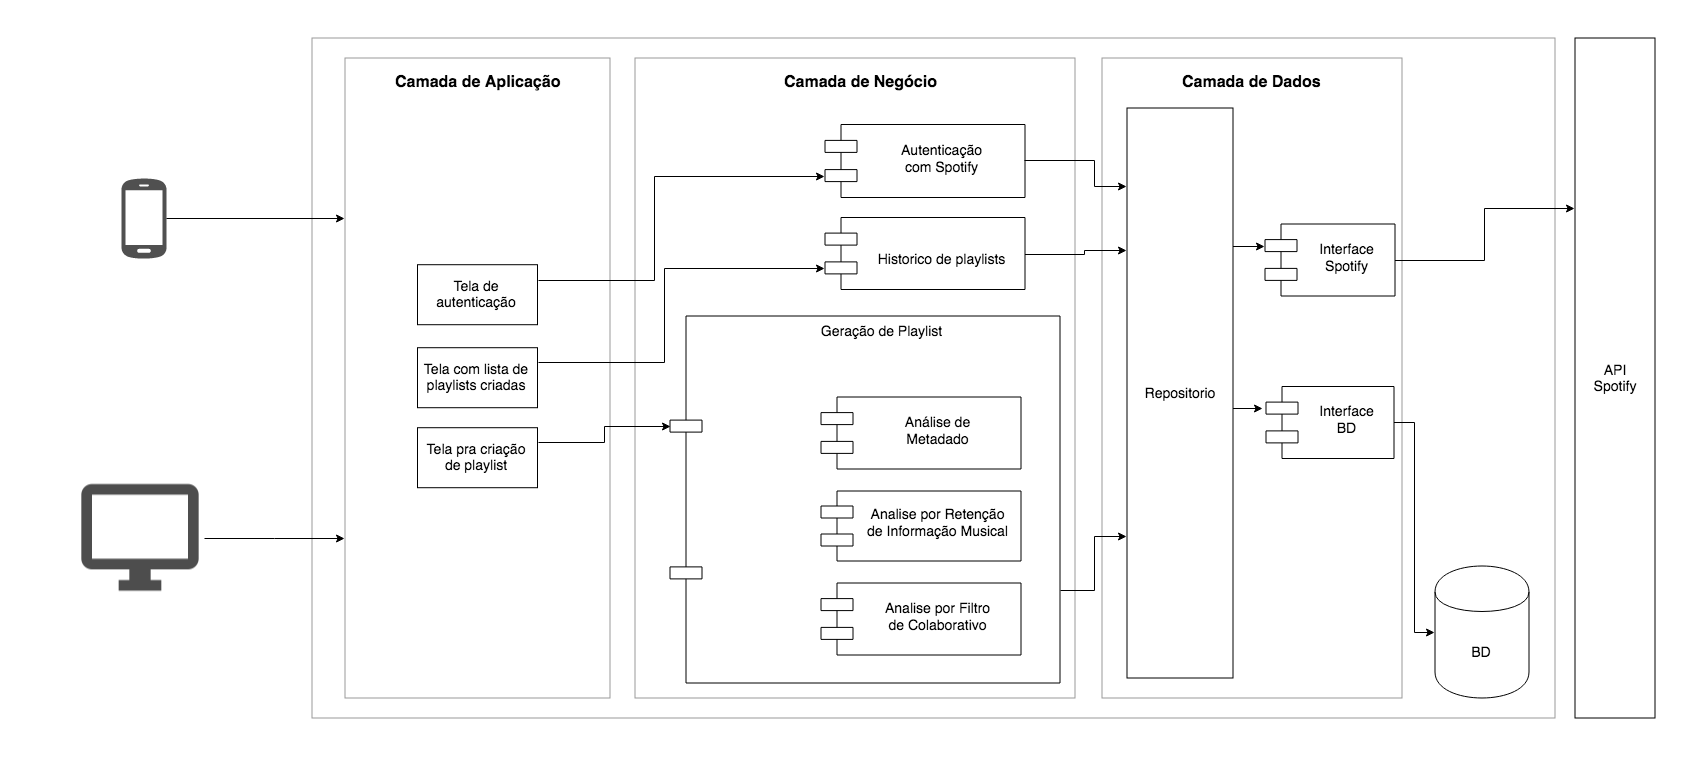
\includegraphics[width=1.0\textwidth]{visao_geral.png}
  \caption{Arquitetura em camadas.}
  \label{fig:arquitetura_em_camadas}
\end{figure}

\subsection{Camada de Aplicação}
A interface do sistema será desenvolvida junto a disciplina PCS3573 (Interação Humano-Computador) em que será usado diversas técnicas para criação e validação das interfaces.
De modo simplificado, serão necessários ao menos 3 telas de interface com o usuário.

\subsubsection{Tela de Autenticação}
Nessa tela, o usuário será levado ao login social da plataforma Spotify, para que possamos obter o acesso aos dados necessários para criar as playlists.

\subsubsection{Tela de Histórico de Playlists}
Nessa tela, o usuário poder ver a lista de playlist em que ele participou, e se desejar, poderá executar novamente qualquer uma das playlists.

\subsubsection{Tela de criação de Playlists}
Nessa tela, o usuário poderá visualizar os outros usuários que participarão da criação de uma playlist. Ele poderá ativar o inicio da geração após todos os integrantes estiverem conectados.

\subsection{Camada de Negócio}
Na camada de negócio, teremos 3 módulos. A seguir iremos descrever cada um deles.

\subsubsection{Módulo de Autenticação com Spotify}
Esse módulo é responsável por realizar o login social com a plataforma Spotify. Também é de sua responsabilidade pedir a permissão do uso dos dados privados a cada usuário.

\subsubsection{Módulo de Histórico de Playlists}
Esse módulo é responsável por trazer as playlist criadas no passado de um determinado usuário.

\subsubsection{Módulo de Geração de Playlists}
Esse módulo é responsável por criar as playlists utilizando os dados de cada um dos usuários.
Internamente ela possui 3 submódulos (Análise de Metadado, Análise por Retenção de Informação Musical, Análise por Filtro Colaborativo). 
Cada submódulo é responsável por uma técnica de sistemas de recomendação. Assim o módulo de geração é responsável por orquestrar a utilização de cada técnica para gerar uma playlist.


\subsection{Camada de Dados}
A camada de dados abstrair o acesso a API do Spotify e ao banco de dados dos sistema. Assim, se por ventura for necessário a mudança da obtenção ou persistência dos dados no decorrer do projeto, as camadas anteriores não sofrerão com o alto acoplamento do sistema.

\subsection{API Spotify}
A API pública do Spotify será a principal fonte de dados sobre os usuários para serem utilizadas nas técnicas de Sistemas de Recomendação. Ela também será utilizada como login social dos usuários nesse sistema.


% ----------------------------------------------------------
% ELEMENTOS PÓS-TEXTUAIS
% ----------------------------------------------------------
\postextual


% ----------------------------------------------------------
% Referências bibliográficas
% ----------------------------------------------------------
\bibliography{abntex2-modelo-references} %% REFERENCIA AO ARQUIVO abntex2-modelo-references.bib
MALBERGIER, Felipe. FILIPPINI, Nazli. SABINO, Rodrigo. “Machine Learning Aplicado a Processamento de Áudio: Distinção Entre Fala e Música”, 2017.\\\\
SALDANHA, Alexandre. OLIVEIRA, Nathália. “Recomendação Dinâmica de Músicas Baseada em Agrupamentos”, 2015.\\\\
BAYLE, Yann. “Deep Learning for Music”, 2017. <https://github.com/ybayle/awesome-deep-learning-music>

% ----------------------------------------------------------
% Glossário
% ----------------------------------------------------------
%
% Consulte o manual da classe abntex2 para orientações sobre o glossário.
%
%\glossary

% ----------------------------------------------------------
% Apêndices
% ----------------------------------------------------------

% ---
% Inicia os apêndices
% ---
% \begin{apendicesenv}

% % Imprime uma página indicando o início dos apêndices
% \partapendices

% % ----------------------------------------------------------
% \chapter{Implementação}
% % ----------------------------------------------------------
 
% \end{apendicesenv}
% % ---


% % ----------------------------------------------------------
% % Anexos
% % ----------------------------------------------------------

% % Inicia os anexos
% \begin{anexosenv}

% \end{anexosenv}




%-----------------------------------------------------------
% INDICE REMISSIVO
%-----------------------------------------------------------
\printindex




\end{document}